\documentclass[11pt]{article}
\usepackage{preamble}

\newcommand{\IconCheck}{[CHECK]}
\newcommand{\IconMic}{[MIC]}
\newcommand{\IconClipboard}{[CLIPBOARD]}
\newcommand{\IconLink}{[LINK]}

\newcommand{\phasetag}[1]{%
  {\small\itshape Tag: #1\par}
}

\newcommand{\phaseitems}[1]{%
  \begin{itemize}[leftmargin=1.5em,itemsep=2pt,topsep=2pt]
  #1
  \end{itemize}%
}

\newcommand{\teacheranswerbox}[2]{%
  \begin{callout}{#1}{calloutgreen}
  {\small #2}
  \end{callout}
}

\newcommand{\qelevengraph}{%
\begin{center}
\begin{tikzpicture}
\begin{axis}[
  width=0.84\linewidth,
  height=2.65in,
  xmin=-5.25,
  xmax=5.25,
  ymin=-80,
  ymax=40,
  axis lines=middle,
  grid=both,
  minor tick num=1,
  xtick={-4,-2,0,2,4},
  ytick={-80,-40,-12,0,40},
  tick label style={font=\small},
  label style={font=\small},
  major grid style={draw=black!25},
  minor grid style={draw=black!10},
  xlabel={$x$},
  ylabel={$y$},
  every axis x label/.style={at={(ticklabel* cs:1)},anchor=west},
  every axis y label/.style={at={(ticklabel* cs:1)},anchor=south},
  clip=false
]
\addplot[tealheader, thick, smooth, domain=-5.2:5.2, samples=250] {x^3 - 2*x^2 - 16*x + 20};
\addplot[warmred, thick, dashed, domain=-5.2:5.2, samples=2] {-12};
\node[font=\small, anchor=west] at (axis cs:1.2,24) {\(f(x)=x^3-2x^2-16x+20\)};
\node[text=warmred, font=\small, anchor=west] at (axis cs:-5.0,-8.5) {\(g(x)=-12\)};
\end{axis}
\end{tikzpicture}
\end{center}
}

\newcommand{\tryitthreeagraph}{%
\begin{center}
\begin{tikzpicture}
\begin{axis}[
  width=0.78\linewidth,
  height=2.45in,
  xmin=-1.5,
  xmax=4.5,
  ymin=-20,
  ymax=30,
  axis lines=middle,
  grid=both,
  minor tick num=1,
  xtick={-1,0,1,2,3,4},
  ytick={-20,-10,0,10,20,30},
  tick label style={font=\small},
  label style={font=\small},
  major grid style={draw=black!25},
  minor grid style={draw=black!10},
  xlabel={$x$},
  ylabel={$y$},
  every axis x label/.style={at={(ticklabel* cs:1)},anchor=west},
  every axis y label/.style={at={(ticklabel* cs:1)},anchor=south},
  clip=false
]
\addplot[tealheader, thick, smooth, domain=-1.5:4.5, samples=250] {2*x^3 - 8*x^2 + 9*x - 9};
\node[font=\small, anchor=west] at (axis cs:0.15,23) {\(f(x)=2x^3-8x^2+9x-9\)};
\end{axis}
\end{tikzpicture}
\end{center}
}

\newcommand{\tryitthreebgraph}{%
\begin{center}
\begin{tikzpicture}
\begin{axis}[
  width=0.78\linewidth,
  height=2.45in,
  xmin=-3.25,
  xmax=3.25,
  ymin=-10,
  ymax=55,
  axis lines=middle,
  grid=both,
  minor tick num=1,
  xtick={-3,-2,-1,0,1,2,3},
  ytick={-10,0,10,20,30,40,50},
  tick label style={font=\small},
  label style={font=\small},
  major grid style={draw=black!25},
  minor grid style={draw=black!10},
  xlabel={$x$},
  ylabel={$y$},
  every axis x label/.style={at={(ticklabel* cs:1)},anchor=west},
  every axis y label/.style={at={(ticklabel* cs:1)},anchor=south},
  clip=false
]
\addplot[tealheader, thick, smooth, domain=-3.2:3.2, samples=250] {x^4 - 3*x^2 - 4};
\node[font=\small, anchor=west] at (axis cs:-3.05,47) {\(f(x)=x^4-3x^2-4\)};
\end{axis}
\end{tikzpicture}
\end{center}
}

\newcommand{\qseventeengraph}{%
\begin{center}
\begin{tikzpicture}
\begin{axis}[
  width=0.78\linewidth,
  height=2.55in,
  xmin=-3.25,
  xmax=4.25,
  ymin=-35,
  ymax=35,
  axis lines=middle,
  grid=both,
  minor tick num=1,
  xtick={-3,-2,-1,0,1,2,3,4},
  ytick={-30,-20,-10,0,10,20,30},
  tick label style={font=\small},
  label style={font=\small},
  major grid style={draw=black!25},
  minor grid style={draw=black!10},
  xlabel={$x$},
  ylabel={$y$},
  every axis x label/.style={at={(ticklabel* cs:1)},anchor=west},
  every axis y label/.style={at={(ticklabel* cs:1)},anchor=south},
  clip=false
]
\addplot[tealheader, thick, smooth, domain=-3.2:4.2, samples=250] {x^3 - x^2 - 4*x - 6};
\node[font=\small, anchor=west] at (axis cs:-3.05,28) {\(f(x)=x^3-x^2-4x-6\)};
\end{axis}
\end{tikzpicture}
\end{center}
}

\newcommand{\storageboxfigure}{%
\begin{center}
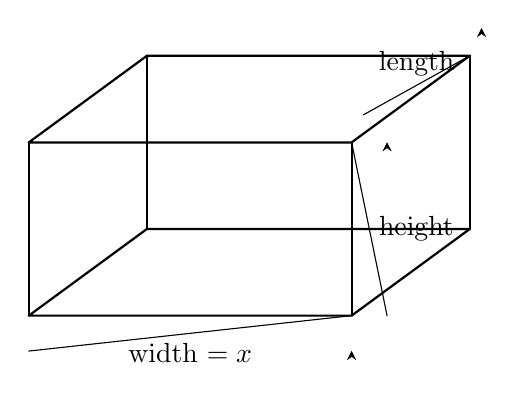
\begin{tikzpicture}[line join=round, line cap=round, >=stealth]
\coordinate (A) at (0,0);
\coordinate (B) at (4.1,0);
\coordinate (C) at (5.6,1.1);
\coordinate (D) at (1.5,1.1);
\coordinate (E) at (0,2.2);
\coordinate (F) at (4.1,2.2);
\coordinate (G) at (5.6,3.3);
\coordinate (H) at (1.5,3.3);

\draw[thick] (A)--(B)--(C)--(D)--cycle;
\draw[thick] (E)--(F)--(G)--(H)--cycle;
\draw[thick] (A)--(E);
\draw[thick] (B)--(F);
\draw[thick] (C)--(G);
\draw[thick] (D)--(H);

\draw[<->] (A)+(0,-0.45) -- node[midway, below] {width \(= x\)} (B)+(0,-0.45);
\draw[<->] (B)+(0.45,0) -- node[midway, right] {height} (F)+(0.45,0);
\draw[<->] (F)+(0.15,0.35) -- node[midway, above] {length} (G)+(0.15,0.35);
\end{tikzpicture}
\end{center}
}

\begin{document}

\packetheading{Lesson 3-5 \textperiodcentered\ Period 3 \textperiodcentered\ Teacher Edition}{Real + Complex Zeros, and Modeling}

\sectionbanner{OBJECTIVES}
{\small
\renewcommand{\arraystretch}{1.25}
\noindent\begin{tabular}{|p{1.8in}|p{4.8in}|}
\hline
\textbf{Math Objective} & Find all zeros (real and complex) of a polynomial function, and use the factored form to model a volume-constrained application. \\ \hline
\textbf{Language Objective} & Students will use the frame ``The zeros are \_\_\_; because \_\_\_, the complex conjugate \_\_\_ must also be a zero.'' to justify complex-zero reasoning. \\ \hline
\textbf{Essential Understanding} & Complex zeros of a polynomial with real coefficients come in conjugate pairs. A cubic model of a physical quantity (volume, profit) can be solved for specific values by factoring and solving. \\ \hline
\end{tabular}
}

\sectionbanner{TOPIC GOALS / ESSENTIAL QUESTION / MATERIALS}
{\small
\renewcommand{\arraystretch}{1.25}
\noindent\begin{tabular}{|p{1.8in}|p{4.8in}|}
\hline
\textbf{Topic Goals} & Students find all zeros (real + complex) of two cubics, then model a Storage Box volume problem end-to-end. Every item is Savvas-sourced. \\ \hline
\textbf{Essential Question} & How do real and complex zeros together describe a polynomial, and how do you use that structure to answer a real-world model? \\ \hline
\textbf{Materials} & Pencils; student packet; calculator (optional). Desmos allowed for Try-It 3 check only, NOT for Practice \#27. \\ \hline
\end{tabular}
}

\begin{callout}{\IconPin\ PRE-FLIGHT --- P3 IS THE DOK-3 SPINE DAY}{calloutpink}
Today's conceptual core is Practice \#27 (Storage Box). It is the single DOK-3 spine and it rehearses Topic 3 Assessment Q\#6 (Lucy's tray).\\
Pace: Try-It 3a/3b (\(\sim\)12 min) \(\rightarrow\) Practice \#17 (\(\sim\)6 min) \(\rightarrow\) Practice \#27 (20 min). Keep Launch tight so Explore gets the full 38 min.\\
Desmos is allowed for Try-It 3 check only. Do NOT use it for Practice \#27.\\
If running tight: follow the Period F cuts below. Never cut Practice \#27.
\end{callout}

\phasetag{bridge from Tuesday}
\frameworkphaseheader{Do Now}{1--2}{5}{%
\phaseitems{
  \item Hand out at door.
  \item Post bridge prompt on board.
  \item Circulate 3 min; cold-call 1 student for one intersection point.
}%
}{%
\phaseitems{
  \item List the intersection points.
  \item Respond to the bridge prompt verbally if called on.
}%
}{%
\phaseitems{
  \item How did you find where the graphs cross?
  \item Bridge: nature of the cubic's coefficients --- why? (Conjugate irrational pair \(\rightarrow\) rational coefficients.)
}%
}{Solo teacher: stand at door, circulate 3 min, cold-call.}

\bankitem{Do Now (3-5-savvas-q11)}{%
At what points do the graphs of \(f(x)=x^3-2x^2-16x+20\) and \(g(x)=-12\) intersect?

\qelevengraph
}{}

\teacheranswerbox{\IconCheck\ ANSWER KEY}{%
\textbf{Answer key (registry):} Solve \(x^3-2x^2-16x+20=-12 \rightarrow x^3-2x^2-16x+32=0 \rightarrow (x-2)(x+4)(x-4)=0.\) Intersection points: \((-4,-12)\), \((2,-12)\), \((4,-12)\).
}

\begin{callout}{\IconLink\ BRIDGE FROM TUESDAY (verbal, posted on board)}{calloutpeach}
A cubic has zeros 2, \(1 + \sqrt{3}\), and \(1 - \sqrt{3}\). What is the nature of its coefficients --- rational, irrational, or complex? Why? (This is Topic 3 Assessment Q\#2 --- no surprises on Thursday.)
\end{callout}

\begin{callout}{\IconLink\ BRIDGE PROMPT --- Expected Answer}{calloutpeach}
``Rational coefficients. The zeros \(1 + \sqrt{3}\) and \(1 - \sqrt{3}\) are irrational conjugates --- when multiplied, \((x-(1+\sqrt{3}))(x-(1-\sqrt{3})) = x^2 - 2x - 2\), which has rational coefficients. Multiplied by \((x-2)\), the full cubic has all rational coefficients.''\\
This is Topic 3 Assessment Q\#2, answer C.
\end{callout}

\begin{callout}{\IconBook\ COMPLEX-ZERO RULES (keep printed on your page)}{calloutgreen}
\textbullet\ A polynomial with real coefficients that has complex zeros has them in CONJUGATE PAIRS.\\
\textbullet\ If \(a + bi\) is a zero, then \(a - bi\) must also be a zero.\\
\textbullet\ A degree-\(n\) polynomial has exactly \(n\) zeros (counting multiplicity). Some may be real, some complex.\\
\textbullet\ Example: if a cubic has a real zero at \(x=4\) and a complex zero \(2 + 3i\), its third zero must be \(2 - 3i\).
\end{callout}

\begin{callout}{\IconWarn\ MODELING RULES (for the Storage Box)}{calloutyellow}
\textbullet\ Set up a factored-form volume function \(V(x) = (\mathrm{expr}_1)(\mathrm{expr}_2)(\mathrm{expr}_3)\).\\
\textbullet\ Each factor is a physical dimension --- label each: length, width, height.\\
\textbullet\ Use the physical constraint (e.g., ``length is greatest'') to decide which factor is which dimension.\\
\textbullet\ To find dimensions at \(V = 10\ \text{ft}^3\), solve the cubic equation --- show all work.
\end{callout}

\phasetag{teacher models Example 3 + brief Example 4}
\frameworkphaseheader{Launch}{2}{12}{%
\phaseitems{
  \item Project Example 3 (real + complex zeros cubic). Think aloud: find one real zero, divide, solve the quadratic.
  \item Brief Example 4 (modeling): 90 sec walk-through of Savvas's storage box --- just the setup, not the solution.
  \item Pause once for 30-sec partner-check on conjugate pair.
}%
}{%
\phaseitems{
  \item Watch silently through Example 3.
  \item Turn-and-talk: ``Why does the quadratic produce the complex pair?''
  \item Write the complex-zero rule in packet margin.
}%
}{%
\phaseitems{
  \item If one real zero is \(x = 4\), what's the next step?
  \item Why does the discriminant being negative produce complex zeros?
  \item How do you know the complex zero's conjugate is also a zero?
}%
}{Project. Think aloud. Do NOT solve Try-Its. Release promptly at minute 17.}

\begin{callout}{\IconMic\ TEACHER SCRIPT}{calloutblue}
1. ``Watch me find all zeros of this cubic. Step 1: guess a real zero by the rational root theorem. Step 2: synthetic divide. Step 3: solve the leftover quadratic.''\\
2. When quadratic's discriminant is negative \(\rightarrow\) ``Now we get complex zeros. They come in conjugate pairs --- so if I get \(2 + 3i\), I also have \(2 - 3i\). That's not a coincidence; it's a rule.''\\
3. Example 4 flash: project the storage box picture. ``Notice the factored form \(V(x) = x(x+3)(x-1)\). We'll unpack this in Explore on the Practice \#27 item.''\\
4. Release: ``You have Try-It 3a, 3b, then Practice \#17, then the big one --- \#27. Manage your time.''
\end{callout}

\phasetag{Think-Pair-Share + DOK-3 modeling}
\frameworkphaseheader{Explore}{2--3}{38}{%
\phaseitems{
  \item 5 laps of circulation across 38 min.
  \item Lap 1: Try-Its 3a/3b. Lap 2: Practice \#17. Laps 3--5: Practice \#27 (\IconStar).
  \item Do not give \#27 answers. Pairs present parts (a)--(d) to each other; then you pick one pair for Share.
}%
}{%
\phaseitems{
  \item Pairs work through Try-It 3a/3b (\(\sim\)12 min), then \#17 (\(\sim\)6 min), then the full 20 min on \#27.
  \item For \#27, write each factor's physical meaning BEFORE solving part (d).
  \item Use sentence frame for the Share.
}%
}{%
\phaseitems{
  \item What are ALL zeros of this polynomial --- real and complex?
  \item How do the factors of \(V(x)\) relate to the box's physical dimensions?
  \item What does the constraint ``length is greatest'' tell you?
  \item For \(V = 10\ \text{ft}^3\), what cubic equation must you solve, and how?
}%
}{Solo teacher: 5 laps of circulation. Press pairs on \#27 part (c) --- physical dimension interpretation is the DOK-3 pivot.}

{\small\itshape Work with a partner. Use the rule cards above. Storage Box (Practice \#27) is the big one --- plan 20 min for it.\par}

\bankitem{Try It 3a (3-5-tryit-3a)}{%
What are all the real and complex zeros of the polynomial function shown in the graph? \(f(x)=2x^3-8x^2+9x-9\).

\tryitthreeagraph
}{}

\teacheranswerbox{\IconCheck\ ANSWER / ANTICIPATED TALK}{%
\textbf{Answer key (registry):} \(x = 3\) (real, from graph + synthetic division), \(x = \dfrac{1 + i\sqrt{5}}{2}\), \(x = \dfrac{1 - i\sqrt{5}}{2}\) (complex, from quadratic formula on the depressed quadratic).
}

\bankitem{Try It 3b (3-5-tryit-3b)}{%
What are all the real and complex zeros of the polynomial function shown in the graph? \(f(x)=x^4-3x^2-4\).

\tryitthreebgraph
}{}

\teacheranswerbox{\IconCheck\ ANSWER / ANTICIPATED TALK}{%
\textbf{Answer key (registry):} Factor as \((x^2-4)(x^2+1) = (x-2)(x+2)(x^2+1)\). Real zeros: \(x = \pm 2\). Complex zeros: \(x = \pm i\).
}

\bankitem{Practice \#17 (3-5-savvas-q17)}{%
What are all the real and complex zeros of the polynomial function shown in the graph? \(f(x)=x^3-x^2-4x-6\).

\qseventeengraph
}{}

\teacheranswerbox{\IconCheck\ ANSWER / ANTICIPATED TALK}{%
\textbf{Answer key (registry):} Zeros: \(x = 3\) (real, from graph), \(x = -1 + i\), \(x = -1 - i\) (from synthetic division by \((x-3)\) then quadratic formula on \(x^2 + 2x + 2\)).
}

\bankitem{Practice \#27 \IconStar\ DOK-3 DRIVER (3-5-savvas-q27)}{%
Model With Mathematics: The height of a rectangular storage box is less than both its length and width. The function \(f(x)=x^3+2x^2-3x\) represents the volume of the rectangular box, where \(x\) represents the width of the box, in feet.

\begin{enumerate}[label=\textbf{(\alph*)}, leftmargin=1.8em, itemsep=2pt, topsep=2pt]
\item Find the factored form of \(f(x)\).
\item Find the zeros of the function.
\item You know \(x\) represents the width of the box. What do the other two factors represent?
\item Find the dimensions of the box when the volume is \(10\ \text{ft}^3\).
\end{enumerate}

\storageboxfigure
}{}

\teacheranswerbox{\IconCheck\ ANSWER / ANTICIPATED TALK}{%
\textbf{Answer key (registry):}\\
\textbf{(a)} \(x(x^2+2x-3) = x(x+3)(x-1)\).\\
\textbf{(b)} Zeros: \(x = 0\), \(x = -3\), \(x = 1\).\\
\textbf{(c)} \((x-1)\) represents the height; \((x+3)\) represents the length.\\
\textbf{(d)} width \(= 2\) ft, height \(= 1\) ft, length \(= 5\) ft.
}

\phasetag{academic conversation + assessment preview}
\frameworkphaseheader{Share / Summary}{2}{7}{%
\phaseitems{
  \item Call 1 pair to the board to present \#27 parts (a)--(d).
  \item Add 30-sec connection: ``Tomorrow's assessment Q\#6 (Lucy's tray) uses the same factored-volume idea.''
  \item Post the exit ticket cue.
}%
}{%
\phaseitems{
  \item Presenting pair walks through each part with sentence frame.
  \item Class signals thumbs up/sideways after each part.
  \item Write the Lucy-tray preview in margin.
}%
}{%
\phaseitems{
  \item Summarize the modeling strategy in one sentence.
  \item What's different between \#27 and tomorrow's Lucy-tray problem? (Different physical setup, same factoring strategy.)
}%
}{Cold-call a pair that struggled earlier (not the strongest). Hold others accountable to listen.}

\begin{sentenceframebox}
\textbf{Sentence Frames}\par
Pair share: ``For the Storage Box, the factored form was \_\_\_. I chose \_\_\_ as the length because \_\_\_. To find \(V = 10\ \text{ft}^3\), I \_\_\_.''\par
Whole class: one pair at random presents Part (a)--(b)--(c)--(d) of \#27.
\end{sentenceframebox}

\phasetag{summary recap (not graded)}
\frameworkphaseheader{Exit Ticket}{1--2}{3}{%
\phaseitems{
  \item Collect at door.
  \item Scan responses to \#3 (assessment prediction). Use tonight to adjust Thursday Do Now emphasis.
}%
}{%
\phaseitems{
  \item Complete 3 sentence stems.
  \item Be honest about \#2 --- the hardest step tells us what to hit Thursday morning.
}%
}{%
\phaseitems{
  \item Did students name a specific step in \#2?
  \item Did they name Topic 3 content (factoring, multiplicity, conjugate pairs, modeling) in \#3?
}%
}{Collect. No grade.}

\begin{callout}{\IconClipboard\ EXIT TICKET --- Student Form}{calloutyellow}
Today I learned that \_\_\_.\\
For the Storage Box, the hardest step was \_\_\_.\\
Thursday's assessment will test \_\_\_.
\end{callout}

\clearpage

\begin{callout}{\IconClock\ PERIOD F --- 45-MIN SHORT VARIANT (Wed only)}{calloutpink}
Period F has 45 min on Wednesday. Apply these cuts:\\
\textbullet\ Launch: skip Example 4 brief (stay on Example 3). Still 12 min.\\
\textbullet\ Explore: 25 min max. DROP Try-It 3b and Practice \#17. Keep Try-It 3a + Practice \#27 only. \#27 is non-negotiable (DOK-3 spine + Thursday-assessment prep).\\
\textbullet\ Share: 5 min (cut from 7). One pair presents \#27 parts (a)+(b) only; (c)+(d) as HW hint.\\
\textbullet\ Exit: 3 min (unchanged).\\
\textbullet\ Optional reinforcement: announce but don't expect completion.
\end{callout}

\begin{callout}{\IconPuzzle\ MODIFICATIONS / SUPPORT FOR IEP STUDENTS}{calloutiep}
\textbullet\ Provide Complex-Zero Rules as a half-sheet cut-out.\\
\textbullet\ For \#27, provide a pre-labeled box sketch (length / width / height slots).\\
\textbullet\ Accept partial solutions on \#27(d) with verbal explanation of which factor is which dimension.
\end{callout}

\begin{callout}{\IconGlobe\ SUPPORTS FOR ELL STUDENTS}{calloutell}
\textbullet\ Sentence frames on student page (do not skip).\\
\textbullet\ Word cards: ``conjugate'' = pair that together gives real numbers; ``imaginary'' = contains \(i = \sqrt{-1}\); ``model'' = equation that describes a real situation.\\
\textbullet\ Pair ELL students with English-dominant partners for Share.\\
\textbullet\ On \#27 part (c), allow verbal responses in students' strongest language before writing.
\end{callout}

\end{document}
